\documentclass[12pt]{article}

\usepackage[margin=1in]{geometry}
\usepackage{amsmath,amsthm,amssymb}
\usepackage{float}
\usepackage{graphicx}

\newcommand{\N}{\mathbb{N}}
\newcommand{\Z}{\mathbb{Z}}

\newenvironment{theorem}[2][Theorem]{\begin{trivlist}
\item[\hskip \labelsep {\bfseries #1}\hskip \labelsep {\bfseries #2.}]}{\end{trivlist}}
\newenvironment{lemma}[2][Lemma]{\begin{trivlist}
\item[\hskip \labelsep {\bfseries #1}\hskip \labelsep {\bfseries #2.}]}{\end{trivlist}}
\newenvironment{exercise}[2][Exercise]{\begin{trivlist}
\item[\hskip \labelsep {\bfseries #1}\hskip \labelsep {\bfseries #2.}]}{\end{trivlist}}
\newenvironment{problem}[2][Problem]{\begin{trivlist}
\item[\hskip \labelsep {\bfseries #1}\hskip \labelsep {\bfseries #2.}]}{\end{trivlist}}
\newenvironment{question}[2][Question]{\begin{trivlist}
\item[\hskip \labelsep {\bfseries #1}\hskip \labelsep {\bfseries #2.}]}{\end{trivlist}}
\newenvironment{corollary}[2][Corollary]{\begin{trivlist}
\item[\hskip \labelsep {\bfseries #1}\hskip \labelsep {\bfseries #2.}]}{\end{trivlist}}


\DeclareMathOperator{\sech}{sech}
\DeclareMathOperator{\csch}{csch}

\begin{document}

\title{CS6210: Homework 1}
\author{Christopher Mertin}
\date{September 6, 2016}
\maketitle

\begin{enumerate}
%%%%%% Problem 1 %%%%%%
\item Carry out calculations similar to those of Example 1.3 for approximating
the derivative of the function $f(x)=e^{-2x}$ evaluated at $x_{0}=0.5$. Observe
similarities and differences by comparing your graph against that in Figure 1.3.

{\bf Solution:}

\begin{figure}[H]
  \centering
  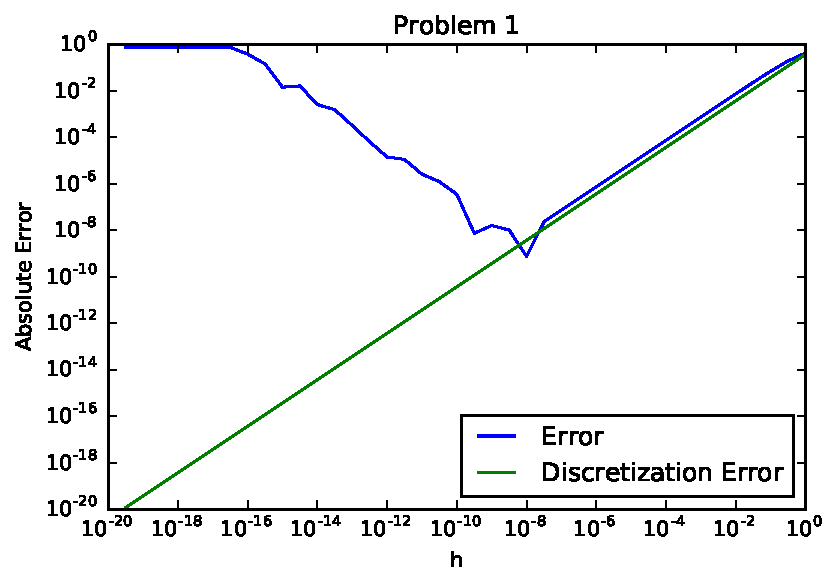
\includegraphics[width=.5\textwidth]{./hw1_prob1.pdf}
  \caption{Refer to {\tt prob1.py}}
  \label{fig:prob1}
\end{figure}

In comparing Figure~\ref{fig:prob1} to Figure 1.3 in the book, it is easy to see
that they represent very similar, almost the same data sets. When $h$ has a relatively
large value, the discretization error dominates the round-off error and causes lots
of problems with the numerical result.

%%%%%% Problem 2 %%%%%%
\item Following Example 1.5, assess the conditioning of the problem of evaluating
\[
  g(x)=\tanh{(cx)} = \frac{e^{cx}-e^{-cx}}{e^{cx}+e^{-cx}}
\]

near $x=0$ as the positive parameter $c$ grows.

{\bf Solution:}

The condition number measures how sensitive the output of a function is to small
changes in the input. It can be calculated by:

\begin{align*}
\text{Condition Number}(g) &= x\frac{g^{\prime}(x)}{g(x)}
\end{align*}

which for the instance of this problem gives us

\begin{align*}
  g(x) &= \frac{e^{cx} - e^{-cx}}{e^{cx}+e^{-cx}} = \frac{\frac{e^{cx}-e^{-cx}}{2}}{\frac{e^{cx}+e^{-cx}}{2}}\\
        &= \frac{\sinh(x)}{\cosh(x)}\\
  g^{\prime}(x) &= c \sech^{2}(cx)\\
                &= \frac{c}{\cosh^{2}(cx)}
\end{align*}

with using these formulas, we can plug it into the definition of the condition
number we get

\begin{align*}
\text{Condition Number}(g) &= x\frac{g^{\prime}(x)}{g(x)} = \frac{cx}{\cosh^{2}(x)\cdot \tanh(cx)}\\
                            &= cx\frac{\cosh(cx)}{\sinh(cx)} = cx\cdot \coth(cx)
\intertext{Where we can take the limit of the condition number as $x$ approaches $0$, giving}
\lim_{x\rightarrow 0} cx\cdot \coth(cx) &= 1
\end{align*}

This shows that the funcion's sensitivity is not dependent upon $c$ and is well conditioned.


%%%%%% Problem 3 %%%%%%
\item The function $f_{1}\left(x_{0},h\right) = \sin\left(x_{0}+h\right) - \sin\left(x_{0}\right)$
can be transformed into another form, $f_{2}\left(x_{0},h\right)$, using the
trigonometric formula
\[
\sin(\phi) - \sin(\psi) = 2\cos\left(\frac{\phi + \psi}{2}\right)\sin\left(\frac{\phi - \psi}{2}\right)
\]
Thus $f_{1}$ and $f_{2}$ have the same values, in exact arithmetic, for any given
argument values $x_{0}$ and $h$.
\begin{enumerate}
\item Derive $f_{2}\left(x_{0},h\right)$

{\bf Solution:}

\[
f_{2}\left(x_{0},h\right) = \sin\left(x_{0} + h\right) - \sin\left(x_{0}\right) = 2\cos\left(x_{0} + \frac{h}{2}\right)\sin\left(\frac{h}{2}\right)
\]
\item Suggest a formula that avoids cancellation errors for computing the approximation
$\left(\left( f\left( x_{0}+h\right) - f\left(x_{0}\right)\right) /h\right)$
to the derivative of $f(x)=\sin(x)$ at $x=x_{0}$. Write a {\sc Matlab} program
that implements your formula and computes an approximation of $f^{\prime}(1.2)$
for $h = \left\{ 10^{-20},10^{-19},\ldots,1\right\}$.

{\bf Solution:}

For $h$ significantly small, the values of $\sin\left(x_{0} + h\right)$ and $\sin\left(x_{0}\right)$
are close as $\sin(x)$ is a smooth trigonometric function. Therefore, there is
a possibiltiy of cancellation occurring for small values of $h$. This can be avoided
by omitting the subtraction and using the equivalent equation stated above. Therefore,
we have

\[
\frac{\sin\left(x_{0}+h\right) - \sin\left(x_{0}\right)}{h} = \frac{2\cos\left(x_{0} + \frac{h}{2}\right)\sin\left(\frac{h}{2}\right)}{h}
\]
\item Explain the difference in accuracy between your results and the results
reported in Example 1.3.

{\bf Solution:}

\begin{figure}[H]
  \centering
  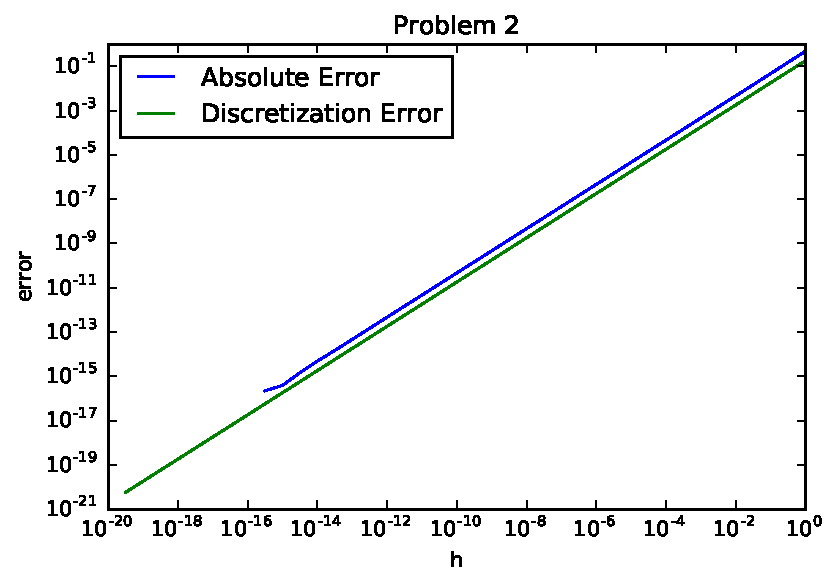
\includegraphics[width=.5\textwidth]{./hw1_prob3.pdf}
  \caption{Refer to {\tt prob3.py}}
  \label{fig:prob3}
\end{figure}

In comparing the two figures, it shows that using the above equation to avoid the
cancellation for small values of $h$ produced correct results as they both agree
at every point. In Figure 1.3, the two curves diverge.
\end{enumerate}

%%%%%% Problem 4 %%%%%%
\item The function $f_{1}(x,\delta) = \cos(x+\delta)-\cos(x)$ can be transformed
into another form, $f_{2}(x,\delta)$, using the trigonometric formula
\[
\cos(\phi) - \cos(\psi) = -2\sin\left(\frac{\phi + \psi}{2}\right)\sin\left(\frac{\phi - \psi}{2}\right)
\]
Thus, $f_{1}$ and $f_{2}$ have the same values, in exact arithmetic, for any given
argument values $x$ and $\delta$.
\begin{enumerate}
\item Show that, analytically, $f_{1}(x,\delta)/\delta$ or $f_{2}(x,\delta)/\delta$
are effective approximations of the function ``$-\sin(x)$'' for $\delta$ sufficiently small.

{\bf Solution:}

This can be done by taking the limit of both functions as $x$ approaches $0$, which gives

\begin{align*}
\lim_{x\rightarrow 0} \frac{\cos(x + \delta) - \cos(x)}{\delta} &= \lim_{x\rightarrow 0} \frac{\cos(x)\cos(\delta) - \sin(x)\sin(\delta) -\cos(x)}{\delta}\\
      &= \lim_{x\rightarrow 0} \frac{\cos(x)\left(\cos(\delta)-1\right) - \sin(x)\sin(\delta)}{\delta}\\
      &= \lim_{x\rightarrow 0}\frac{\cos(x)\left(\cos(\delta)-1\right)}{\delta} - \lim_{x\rightarrow 0} \frac{\sin(x)\sin(\delta)}{\delta}\\
      &= \cos(x)\lim_{x\rightarrow 0}\frac{\cos(\delta) - 1}{\delta} - \sin(x)\lim_{x\rightarrow 0}\frac{\sin(\delta)}{\delta}\\
      &= 0\cdot \cos(x) - 1 \cdot \sin(x) = -\sin(x)
\end{align*}
\item Derive $f_{2}(x,\delta)$

{\bf Solution:}

\[
f_{2}(x,\delta) = \cos(x + \delta) - \cos(x) = -2\sin\left(\frac{2x + \delta}{2}\right)\sin\left(\frac{\delta}{2}\right)
\]
\item Write a {\sc Matlab} script which will calculate $g_{1}(x,\delta) = f_{1}(x,\delta)/\delta + \sin(x)$
and $g_{2}(x,\delta) = f_{2}(x,\delta)/\delta + \sin(x)$ for $x = 3$ and $\delta = 10^{-11}$.

{\bf Solution:}

Refer to {\tt prob4.py}

{\tt g1 = -4.4060023643432977e-07}

{\tt g2 = 4.949957110866876e-12}

\item Explain the difference in the results of the two calculations.

{\bf Solution:}

The values of $g_{1}$ and $g_{2}$ should converge to zero as $\delta$ goes to zero.
As can be seen in the results, $g_{2}$ is closer to zero so it therefore provides
a better approximation of the derivative of $\cos(x)$.

\end{enumerate}

%%%%%% Problem 5 %%%%%%
\item Consider the approximation of the first derivative
\[
f^{\prime}(x) \approx \frac{f(x+h)-f(x)}{h}
\]
The {\em truncation error} for this formula is $\mathcal{O}(h)$. Suppose that the
absolute error in evaluating the function $f$ is bounded by $\epsilon$ and
let us ignore the errors generated in basic arithmetic operations.
\begin{enumerate}
\item Show that the total computational error (truncation error and rounding combined)
is bounded by
\[
\frac{Mh}{2} + \frac{2\epsilon}{h}
\]
where $M$ is a bound on $\left| f^{\prime\prime}(x)\right|$.

{\bf Solution:}

In order to solve this, the following terms need to be defined:

\begin{itemize}
\item $f^{\prime}$: The {\em exact} derivative of $f$
\item $\widetilde{f^{\prime}}$: The value of $f^{\prime}$ with the discretization error
\item $\widetilde{f^{\prime}_{\star}}$: The value of $f^{\prime}$ with discretization {\em and} rounding error
\item $\widetilde{f_{\star}}$: The value of $f$ with discretization {\em and} rounding error
\end{itemize}

Now that the notation is defined. We can approximate the first derivative of a
function with a Taylor Series expansion about 0. In doing so, we get

\begin{align*}
&f\left(x_{0} + h\right)  = f\left(x_{0}\right) + hf^{\prime}\left(x_{0}\right) + \frac{h^{2}}{2}f^{\prime \prime}\left(x_{0}\right) + \ldots\\
&\left| f^{\prime}\left(x_{0}\right) - \frac{f\left(x_{0}+h\right) - f\left(x_{0}\right)}{h}\right| \leq h\frac{f^{\prime\prime}\left(x_{0}\right)}{2} \leq h\frac{M}{2}
\end{align*}

which can be rewritten using the new notation defined above as

\begin{align*}
\left| f^{\prime} - \widetilde{f^{\prime}} \right| \leq h\frac{M}{2}
\end{align*}

From the definition of the {\em abolsute error} $(\xi)$, we get the absolute error on $f$ being bounded by $\epsilon$

\[
\xi = \left| f - \widetilde{f_{\star}} \right| < \epsilon
\]

Following this, we have

\begin{align*}
\left| f^{\prime} - \widetilde{f^{\prime}_{\star}} \right| &= \left| f^{\prime} - \widetilde{f^{\prime}} + \widetilde{f^{\prime}} -\widetilde{f^{\prime}_{\star}} \right|\\
&< \left| f^{\prime} - \widetilde{f^{\prime}} \right| + \left| \widetilde{f^{\prime}} - \widetilde{f^{\prime}_{\star}} \right|\\
&< h\frac{M}{2} + \left| \widetilde{f^{\prime}} - \widetilde{f^{\prime}_{\star}} \right|
\end{align*}

From looking at the defintions of the terms defined above, we can say that
$\left| \widetilde{f^{\prime}} - \widetilde{f^{\prime}_{\star}} \right| $ is equal
to the {\em rounding error} which is equal to $\frac{2\epsilon}{h}$. Therefore,
we proved what we were asked to.

\item What is the value of $h$ for which the above is minimized?

{\bf Solution:}

In finding the extremas, we can take the derivative of the funciton, set it equal to zero, and then solve the system

\begin{align*}
\frac{d}{dh}\left(h\frac{M}{2} + \frac{2\epsilon}{h}\right) &= \frac{M}{2} - \frac{2\epsilon}{h^{2}}\\
\frac{M}{2} - \frac{2\epsilon}{h^{2}} &= 0\\
h &= 2\sqrt{\frac{\epsilon}{M}}
\end{align*}

\item The rounding unit we employ is approximately equal to $10^{-16}$. Use this
to explain the behavior of the graph in Example 1.3. Make sure to explain the shape
of the graph as well as the value where the apparent minimum is attained.

{\bf Solution:}

Example 1.3 gives $f(x) = \sin(x)$, so $f^{\prime\prime}(x) = -\sin(x)$. Since $M$ is a bound
for $\left| -\sin(x)\right|$, it is 1. Using the given tolerance value of $\epsilon$, we can solve
for $h$, giving

\begin{align*}
\epsilon &= 10^{-16}\\
h &= 2\sqrt{\frac{\epsilon}{M}} = 2\cdot 10^{-8}
\end{align*}

\item It is not difficult to show, using Taylor expansions, that $f^{\prime}(x)$ can
be approximated more accurately (in terms of truncation error) by
\[
f^{\prime}(x) \approx \frac{f(x+h) - f(x-h)}{2h}
\]
For this approximation, the truncation error is $\mathcal{O}\left(h^{2}\right)$.
Generate a graph similar to Figure 1.3 for the same function and the same value
of $x$, namely, for $\sin(1.2)$, and compare the two graphs. Explain the meaning
of your results.

{\bf Solution:}

\begin{figure}[H]
  \centering
  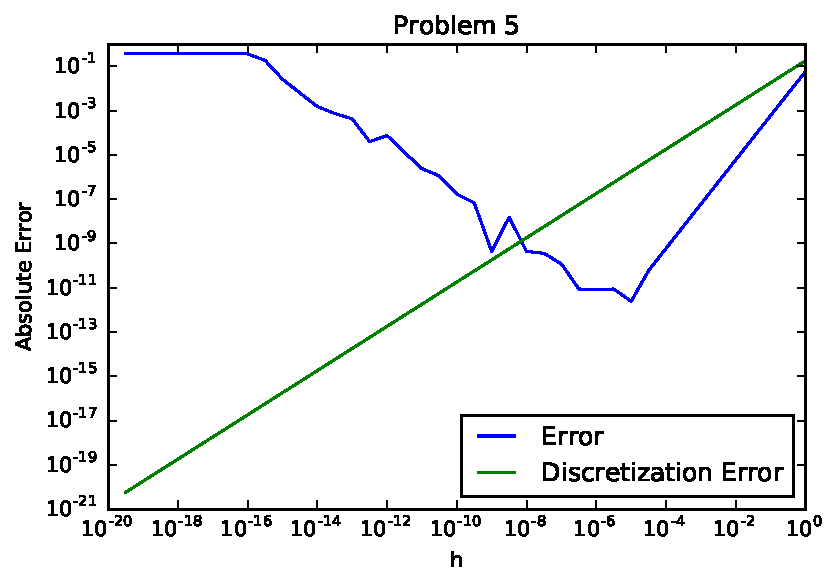
\includegraphics[width=.5\textwidth]{./hw1_prob5.pdf}
  \caption{Refer to {\tt prob5.py}}
  \label{fig:prob5}
\end{figure}

In comparing Figure 1.3 and Figure \ref{fig:prob5}, it is easy to see that the
combined effect of the discretization and round off errors produces a smaller
absolute error in using a central difference scheme when compared to a forward
difference scheme. This is to be expected, as the error is $\mathcal{O}\left(h^{2}\right)$
for the central difference and $\mathcal{O}(h)$ for the forward difference.
\end{enumerate}

%%%%%% Problem 6 %%%%%%
\item In the statistical treatment of data one often needs to compute the quantities
\[
\bar{x} = \frac{1}{n}\sum_{i=1}^{n}x_{i},\quad \sigma^{2}=\frac{1}{n}\sum_{i=1}^{n}\left(x_{i}-\bar{x}\right)^{2}
\]
where $\left\{ x_{1}, x_{2}, \ldots, x_{n}\right\}$ are the given data. Assume that $n$
is large, say, $n = 10\,000$. It is easy to see that $\sigma^{2}$ can also be written as
\[
\sigma^{2} = \frac{1}{n}\sum_{i=1}^{n} x_{i}^{2} - \bar{x}^{2}
\]
\begin{enumerate}
\item Which of the two methods to calculate $\sigma^{2}$ is cheaper in terms of
overall computational cost? Assume $\bar{x}$ has already been calculated and give
the operation counts for these two options.

{\bf Solution:}

The first equation of $\sigma^{2}$ requires $n$ squares, $n$ subtractions, $n$ additions, and 1 division.
This results in an overall computational cost of $\mathcal{O}(3n+1)$, while the second
equation, assuming $\bar{x}^{2}$ is {\em not} precomputed,
of $\sigma^{2}$ requires $n+1$ squares, 1 subtraction, $n$ additions, and 1 division,
resulting in an overall complexity of $\mathcal{O}(2n+2)$.

\item Which of the two methods is expected to give more accurate results for
$\sigma^{2}$ in general?

{\bf Solution:}

The first equation has $n$ subtractions while there is only a single subtraction
in the second equation. Therefore, there will be less cancellation error in the
second equation, so it should produce a more accurate answer.

\item Give a small example, using a decimal system with precision $\tau = 2$ and
numbers of your choice, validate your claims.

{\bf Solution:}

Work goes here
\end{enumerate}
\end{enumerate}

%\begin{proof}
%Blah, blah, blah.  Here is an example of the \texttt{align} environment:
%Note 1: The * tells LaTeX not to number the lines.  If you remove the *, be sure to remove it below, too.
%Note 2: Inside the align environment, you do not want to use $-signs.  The reason for this is that this is already a math environment. This is why we have to include \text{} around any text inside the align environment.
%\begin{align*}
%\sum_{i=1}^{k+1}i & = \left(\sum_{i=1}^{k}i\right) +(k+1)\\
%& = \frac{k(k+1)}{2}+k+1 & (\text{by inductive hypothesis})\\
%& = \frac{k(k+1)+2(k+1)}{2}\\
%& = \frac{(k+1)(k+2)}{2}\\
%& = \frac{(k+1)((k+1)+1)}{2}.
%\end{align*}
%\end{proof}

\end{document}
